\chapter{Resultaten}%
In dit hoofdstuk word er dieper in de onderzoeksresultaten van dit onderzoek gedelft. Alle resultaten zijn verkregen door de applicatie te testen via een fysiek toestel(Iphone Xr, IOS 17.0). Alle testen zijn ook systematisch 100 keer overlopen voor een correcter resultaat. Elke afbeelding in dit hoofdstuk bevatten rechtstreekse resultaten vanuit de XCode Profiler. Bij deze afbeeldingen word er ook een kort woordje uitleg gedaan die de resultaten beschrijven.

\label{ch:resultaten}
\section{CPU verbruik}
Voor het meten van het CPU verbruik tijdens het testen van verschillende methoden van data-overdracht is de Xcode profiling tool gebruikt met als template de CPU profiler. Met deze tool is gemeten hoeveel Mc(Mega cycles) de app vereist heeft van de CPU per type van data-overdracht. 

\subsubsection{binding}
Uit de tabel blijkt dat wanneer we een binding gebruiken om een groot object door te geven aan een view, en we maken een aanpassing in die view, dit ongeveer 14,08 mega cycli van de CPU vereist.
\begin{figure}[htbp]
    \centering
    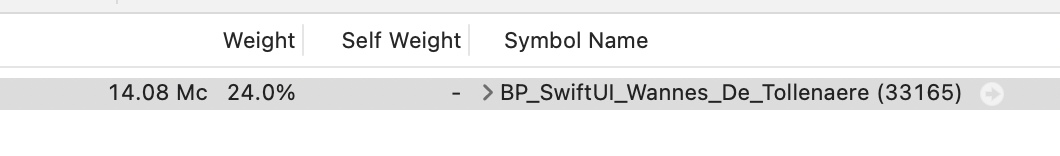
\includegraphics[width=1\textwidth]{BP_CpuUsageBinding} 
    \caption{CPU gebruik van binding}
    \label{fig:cpuBinding}
\end{figure}

\subsubsection{environment}
Uit de tabel blijkt dat het gebruik van Environment om een groot object door te geven aan een view, en het vervolgens aanpassen van dat object, ongeveer 250,08 kilocycli van de CPU vereist.
\begin{figure}[htbp]
    \centering
    
\includegraphics[width=1\textwidth]{BP_CpuUsageEnvironment} 
    \caption{CPU gebruik van environment}
    \label{fig:cpuEnvironment}
\end{figure}

\subsubsection{environmentObject}
Uit de tabel blijkt dat het gebruik van een environmentObject om een groot object door te geven aan een view, en het vervolgens aanpassen van dat object, ongeveer 17,13 mega cycli van de CPU vereist.
\begin{figure}[htbp]
    \centering
    
\includegraphics[width=1\textwidth]{BP_CpuUsageEnvironmentObject} 
    \caption{CPU gebruik van environmentObject}
    \label{fig:cpuEnvironmentObject}
\end{figure}

\subsubsection{observable}
Uit de tabel blijkt dat wanneer we een Observable gebruiken om een groot object door te geven aan een view, en we vervolgens een aanpassing aan dat object in die view maken, dit ongeveer 19,45 mega cycli van de CPU vereist.
\begin{figure}[htbp]
    \centering
    
\includegraphics[width=1\textwidth]{BP_CpuUsageObservable} 
    \caption{CPU gebruik van een Observable}
    \label{fig:cpuObservable}
\end{figure}\

\subsubsection{observableObject}
Uit de tabel blijkt dat wanneer we een observableObject gebruiken om een groot object door te geven aan een view, en we vervolgens een aanpassing aan dat object in die view maken, dit ongeveer 17,82 mega cycli van de CPU vereist.
\begin{figure}[htbp]
    \centering
    
\includegraphics[width=1\textwidth]{BP_CpuUsageObservedObject} 
    \caption{CPU gebruik van observableObject}
    \label{fig:cpuObservedObject}
\end{figure}

\subsubsection{observableObject}
Uit de tabel blijkt dat het simpelweg doorgeven van een groot object aan een view zonder speciale annotaties, en zonder er vervolgens aanpassingen op te maken, gemiddeld 2,00 mega cycli van de CPU verbruikt.
\begin{figure}[htbp]
    \centering
    
\includegraphics[width=1\textwidth]{BP_CpuUsageWithoutPropertyWrapper} 
    \caption{CPU gebruik van een view zonder property wrappers}
    \label{fig:cpuWithoutPropertyWrapper}
\end{figure}

Uit voorgaande resultaten kan worden afgeleid dat Environment voordelen biedt op het gebied van CPU-verbruik. Deze conclusie is echter niet volledig vergelijkbaar met andere property wrappers, omdat Environment een specifieke functie vervult. We kunnen daarom concluderen dat Binding het minste CPU-verbruik vereist om objecten door te geven aan een SwiftUI-view. Daarnaast kunnen we uit de voorgaande tabellen afleiden dat de nieuwere observable macro zwaarder is voor de CPU dan alle andere annotaties.

\newpage
\section{Property updates}
Voor het meten van het aantal updates van verschillende view property's tijdens het testen van verschillende methoden van data-overdracht is de Xcode profiling tool gebruikt met als template de Swift-UI profiler. Met deze tool is het aantal updates waargenomen dat elke datatype heeft gedaan na 101 keer een aanpassing door te voeren op een groot object en dat aan de overdrachtsmethode te koppelen. Na deze test uit te voeren kan opgemaakt worden dat Binding, ObservedObject en EnvironmentObject de property 202 keer hebben bijgewerkt, terwijl Observable en Environment de property slechts 101 keer hebben bijgewerkt. Dit verschil in updatefrequentie heeft invloed op de nauwkeurigheid en consistentie van de state van de applicatie, wat belangrijk is voor een responsieve gebruikerservaring. Echter, te vaak updaten kan leiden tot een hogere CPU-belasting en minder efficiënte prestaties.

\subsection{Snellere reactiesnelheid}
Binding, ObservedObject en EnvironmentObject passen de property bij elke wijziging tweemaal aan, wat zorgt voor een snellere en consistenter bijgewerkte state. Deze methoden zijn geschikt voor applicaties waarbij real-time gegevensuitwisseling en een directe reactie op veranderingen essentieel zijn, zoals een chatapplicatie of een live-dashboard.

\subsection{Tragere reactiesnelheid}
Daarentegen voeren Observable en Environment slechts één update per aanpassing uit, wat kan resulteren in minder efficiënte of langzamere reacties op veranderingen. Deze methoden kunnen beter geschikt zijn voor applicaties waar updates minder frequent zijn of waar de responsietijd minder kritisch is, zoals een notitie-app of een takenbeheer-app.


\begin{figure}[htbp]
    \centering
    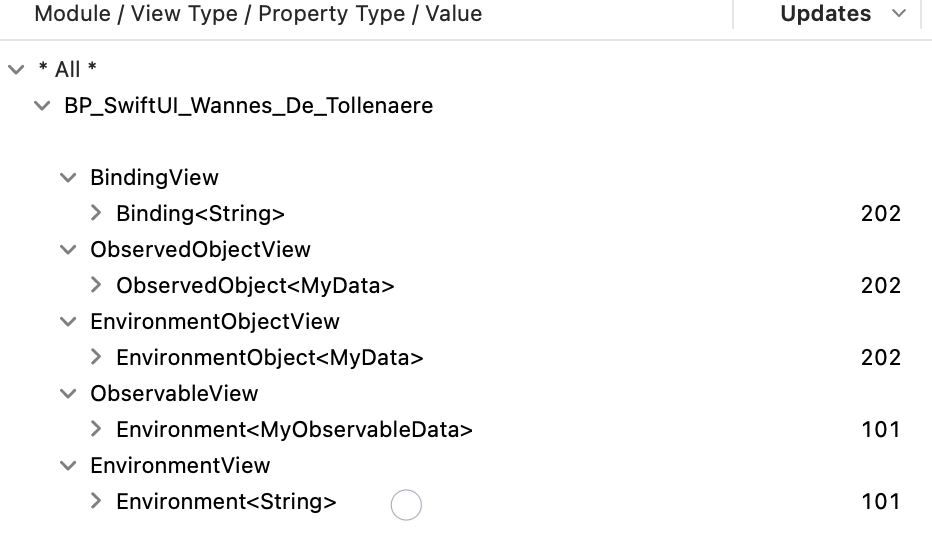
\includegraphics[width=1\textwidth]{BP_ViewPropertyUpdates} 
    \caption{Aantal keren dat de property's geupdate zijn bij het 101 keer opnieuw toewijzen}
    \label{fig:propertyUpdates}
\end{figure}

\newpage
\section{View refresh time}
Voor het meten van het gemiddelde view refresh times van SwiftUI Views tijdens het testen van verschillende methoden van data-overdracht is de Xcode profiling tool gebruikt met als template de SwiftUI profiler. De resultaten zijn waargenomen door een view aan te maken, de data door te geven volgens de methode die aangegeven is. Vervolgens de data updaten. Dit 100x herhalen voor elk type View. Ten slotte de gemiddelde tijdswaarden aflezen in de Xcode profiler.

\begin{figure}[htbp]
    \centering
    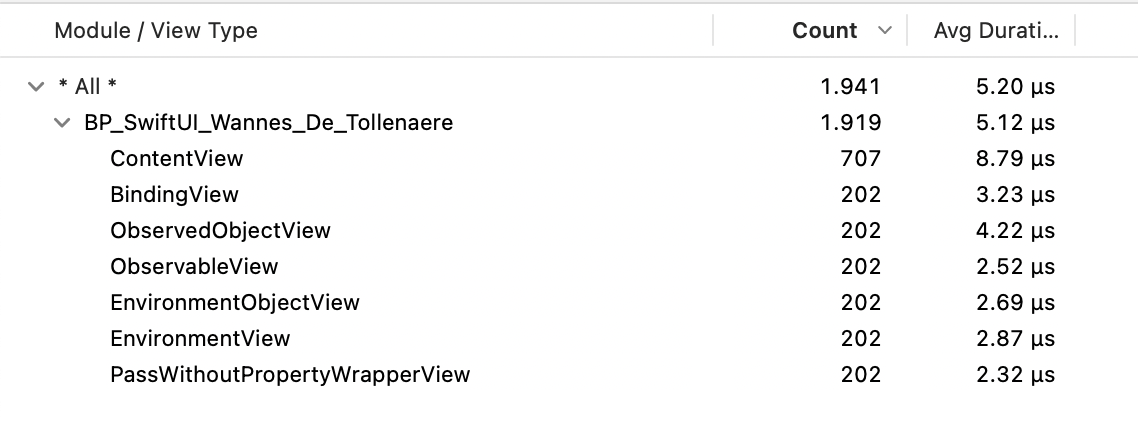
\includegraphics[width=1\textwidth]{BP_ViewRefreshCountAvgDuration} 
    \caption{Gemiddelde duratie voor de view om in te laden per property type}
    \label{fig:propertyRefreshDuration}
\end{figure}

\subsection{Observable en EnvironmentObject}
Deze methoden laten de snelste refresh times zien, met respectievelijk 2.52 en 2.69 microseconden. Dit laat zien dat deze benaderingen efficiënter zijn in het updaten van de UI wanneer de onderliggende data verandert. Dit kan worden toegeschreven aan de geoptimaliseerde manier waarop Observable en EnvironmentObject werken in SwiftUI, waarbij Observable expliciete meldingen van datawijzigingen mogelijk maakt, en EnvironmentObject een efficiënte, globale benadering biedt.

\subsection{Environment}
De gemiddelde refresh time voor Environment (2.87 microseconden) ligt dicht bij die van Observable en EnvironmentObject. Dit duidt op een vergelijkbare efficiëntie, maar mogelijk iets minder optimaal vanwege de bredere reikwijdte van het gebruik van Environment in SwiftUI-applicaties.

\subsection{Binding}
Met een gemiddelde refresh time van 3.23 microseconden is binding iets minder efficiënt dan Observable en EnvironmentObject. Dit kan worden verklaard door de manier waarop binding werkt, wat meer overhead kan introduceren in vergelijking met de directe datawijzigingen van Observable en EnvironmentObject.

\subsection{ObservedObject}
Deze methode laat de traagste refresh time zien (4.22 microseconden) in vergelijking met de andere benaderingen. Dit kan duiden op een hoger overheadniveau of minder optimalisaties in de manier waarop ObservedObject wordt gebruikt voor het volgen en updaten van UI-componenten.

\paragraph{Bevindingen}
Over het algemeen lijken Observable en EnvironmentObject de meest efficiënte benaderingen voor het snel updaten van de UI in SwiftUI-applicaties. Binding en ObservedObject zijn minder efficiënt en kunnen mogelijk extra overhead toevoegen. Deze bevindingen kunnen ontwikkelaars helpen bij het kiezen van de meest geschikte data-binding benadering voor hun SwiftUI-applicaties.



